\begin{definicja}[Algorytm]\label{def:algorytm}
Zbiór jednoznacznie określonych reguł lub zadań obliczeniowych prowadzących w skończonej ilości kroków do rozwiązania pewnego problemu \cite{IEEE}.
\end{definicja}


Określone w ten sposób zadania obliczeniowe są z reguły względem siebie niezależne. Pewne z zadań mogą być wykonywane równolegle, inne muszą być wykonywane sekwencyjnie, jedno po drugim. Wobec tego algorytm może być określony częściowo równolegle, częściowo sekwencyjnie.


Podstawowymi elemetami określającymi dowolny algorytm są:
\begin{enumerate}
\item zadania do wykoniania,
\item zależności pomiędzy zadaniami polegające na określeniu czy 
dane wyjściowe któregoś z zadań nie są danymi wejściowymi dla innego zadania,
\item zbiór danych wejściowych wymaganych przez algorytm,
\item zbiór danych wyjściowych otrzymywanych po wykonania algorytmu.
\end{enumerate}

%Na podstawie niezależności zadań obliczeniowych algorytmy możemy %podzielić na pięć klas \cite{APC2011}:
%\begin{enumerate}
%\item Algorytmy szeregowe
%\item Algorytmy równoległe
%\item Algorytmy szeregowo--równoległe (SPA, Serial--Parallel %Algorithms)
%\item Algorytmy nieszeregowo--równoległe (NSPA, Nonserial--%Parallel Algorithms)
%\item Algorytmy regularno-iteracyjne (RIA, Regular--Iterative %Algorithms)
%\end{enumerate}

\begin{definicja}[Algorytm sekwencyjny]\label{def:algorytm_sekwencyjny}
\textbf{Algorytm sekwencyjny} (rys.  \ref{fig:sequential}) jest ciągiem dokładnie sprecyzowanych zadań obliczeniowych \(T_i,\, i\in\mathbb{N}\) rozwiązujących dany problem, tj. wyznaczających dane wyjściowe na podstawie danych wejściowych. Zakłada się, że w algorytmie sekwencyjnym zadania wykonywane są przez jeden procesor.

\end{definicja}

\begin{figure}[h]
\centering
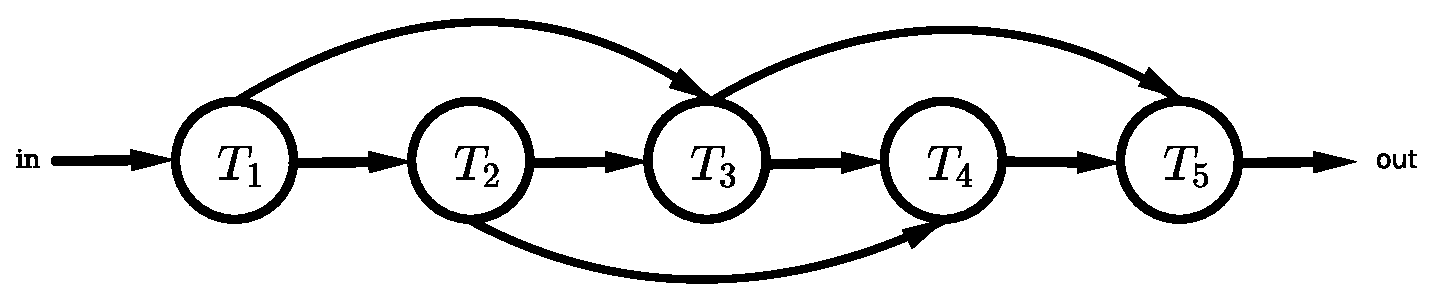
\includegraphics[width=29em]{images/Rys2.eps}
\caption{Algorytm sekwencyjny}
\label{fig:sequential}
\end{figure}

W celu rozwiązania problemu za pomocą większej liczby procesorów należy go zdekomponować na podproblemy, które mogą być rozwiązane równolegle. Każdy z podproblemów rozwiązywany jest przez odrębny algorytm będący składową algorytmu równoległego.


\begin{definicja}[Równoległość]\label{def:rownoleglosc}
\textbf{Równoległość} w odniesieniu do oprogramowania jest to symultaniczny transfer, występowanie albo przetwarzanie poszczególnych części pewnej całości, takich jak bity składające się na znak albo znaki pewnego słowa, używając osobnych urządzeń dla ich różnych części \cite{IEEE}.
\end{definicja}


\begin{definicja}[Algorytm równoległy]\label{def:algorytm_rownolegly}
\textbf{Algorytmem równoległym} (rys. \ref{fig:parallel}) nazywamy każdy algorytm, w którym spośród określonych w nim zadań \(T_1\), \(T_2\), \(\dots\), \(T_n\) co najmniej dwa zadania \(T_i\), \(T_j\), \(i\neq j\) dzięki ich wzajemnej niezależności, mogą być wykonane równocześnie \cite{APC2011}.\\
\end{definicja}

\begin{figure}[h]
\centering
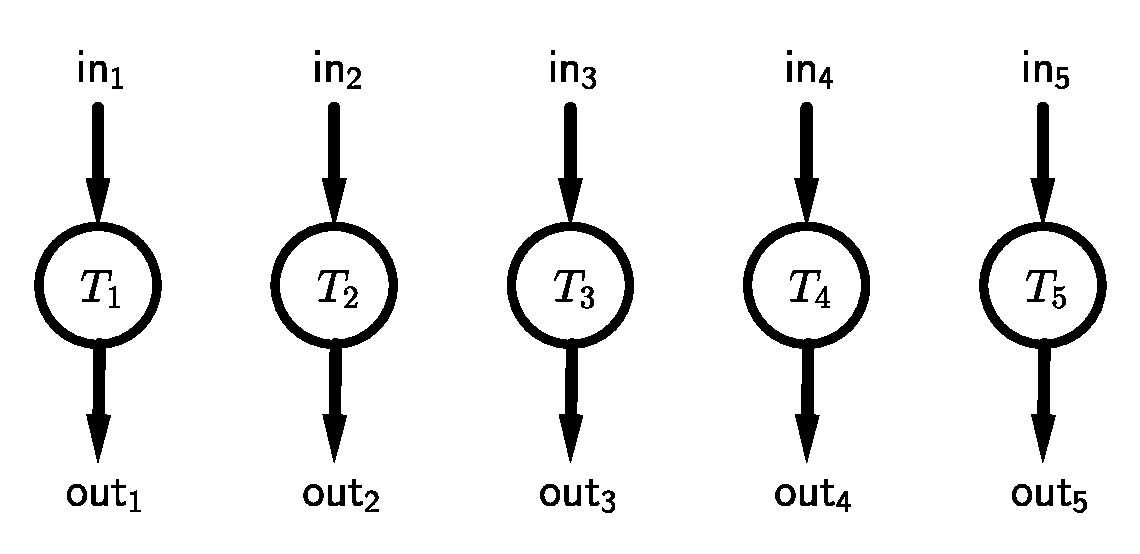
\includegraphics[width=23em]{images/Rys1.eps}
\caption{Algorytm równoległy}
\label{fig:parallel}
\end{figure}

\subsection{Architektury równoległe}

\begin{definicja}[Architektura równoległa]\label{def:arch_rownolegla}
\textbf{Architektura równoległa} jest to architektura wieloprocesorowa, na której można wykonywać przetwarzanie równoległe \cite{IEEE}.
\end{definicja}

Algorytmy równoległe i architektury równoległe są ze sobą blisko spokrewnione. Równoległość może być zaimplementowana na wielu poziomach używając technik sprzętowych i programowych.
\begin{enumerate}
\item{Równoległość na poziomie danych (\emph{Data-level parallelism}), gdzie pracujemy na wielu bitach danych lub na wielu danych jednocześnie.}
\item{Równoległość na poziomie instrukcji (\emph{Instruction-level parallelism}, ILP), gdzie jednocześnie procesor może wykonać więcej niż jedną instrukcję.}
\item{Równoległość na poziomie wątków (\emph{Thread-level parallelism}, TLP). Wątek jest częścią programu, która współdzieli zasoby procesora z innymi wątkami. W TLP wiele programowych wątków jest uruchamianych jednocześnie na jednym bądź wielu procesorach.}
\item{Równoległość na poziomie procesów (\emph{Process-level parallelism}). Proces to program, który jest uruchomiany na komputerze. Rezerwuje on własne zasoby komputera, takie jak przestrzeń pamięciową i rejestry.\cite{APC2011}}
\end{enumerate}

\begin{przyklad}
Prostym przykładem algorytmu równoległego jest serwer siecowy, który każde zapytanie przychodzące przetwarza niezależnie od innych zapytań. Innym przykładem są wielozadaniowe systemy operacyjne radzące sobie z jednoczesną obsługą kilku uruchomionych programów.
\end{przyklad}



\subsubsection{Klasyfikacja Flynna}
Architektury komputerowe można podzielić na klasy ze względu na liczbę równolegle wykonywanych instrukcji oraz dostępnych strumieni danych. Klasyfikację taką (rys. \ref{fig:flynn} zaproponował Michael J. Flynn w 1966 roku i przyjęła ona swoją nazwę od jego nazwiska (rys. \ref{fig:flynn})

\begin{figure}
\centering
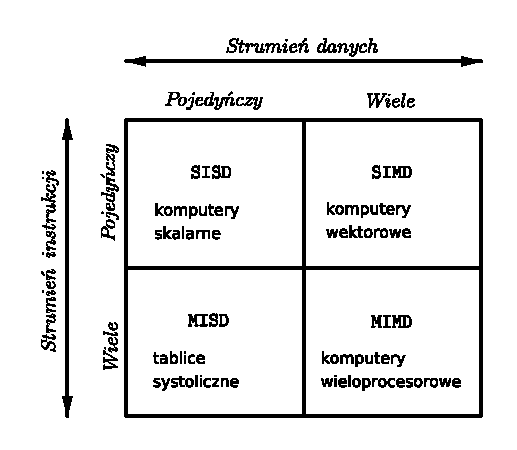
\includegraphics[width=24em]{images/flynn.eps}
\caption{Klasyfikacja Flynna}
\label{fig:flynn}
\end{figure}

\paragraph{SISD.}
Klasa SISD (ang. \emph{Single Instruction, Single Data}) odnosi się do komputerów wykonujących pojedyńczy strumieniem instrukcji i przetwarzających pojedyńczy strumień danych. Są to komputery całkowicie sekwencyjne, które nie wykonują żadnych obliczeń równoległych.
\paragraph{SIMD.}
Klasa SIMD (ang. \emph{Single Instruction, Multiple Data}) odnosi się do komputerów obsługujących pojedyńczy strumień instrukcji i przetwarzających wiele strumieni danych. Na różnych zbiorach danych wykonywane są te same operacje. Jako przykład takiej architektury warto wymienić przede wszystkim wczesne komputery macierzowe (nazywane niekiedy wektorowymi) ze wspólną pamięcią i macierzą jednostek przetwarzających nadzorowanych przez jednostkę sterującą takie jak komputer ILLIAC IV wykorzystywany przez NASA do ,,podboju kosmosu''.
\paragraph{MISD.}
Klasa MISD (ang. \emph{Multiple Instruction, Single Data}) 
odnosie się do komputerów wykonujących jednocześnie wiele instrukcji przetwarzających jeden współny strumien danych. Przykładem takiej architektury jest tablica systoliczna\footnote{Nazwa pochodzi od skurczu mięśni serca przez analogię ,,pompowani'' danych do jednostek przetwarzających na wzór krwi w naczyniach krwionośnych}. Tablica systoliczna jest to układ prostych jednostek przetwarzających połączonych w sieć z sąsiadującymi jednostkami, które synchronicznie wykonują pewne elementarne operacje obliczeniowe.
\paragraph{MIMD.}
Klasa MIMD  (ang. \emph{Multiple Instruction, Multiple Data})
odnosi się do komputerów równolegle wykonujących wiele instrukcji z których każda przetwarza własne strumienie danych.



%
%\begin{definicja}[Algorytmy szeregowo--równoległe]
%
%\end{definicja}
%
%\begin{definicja}[Algorytmy nieszeregowo--równoległe]
%\end{definicja}
%
%\begin{definicja}[Algorytmy regularno--iteracyjne]
%Algorytmy tej klasy reprezentowane za pomocą grafów zależności wyrażają pewien pewien ustalny schemat postępowania.
%\end{definicja}